%!TEX root=../main.tex
% Chapter Template

\chapter{Experimental Validation} % Main chapter title

\label{Chapter5} % Change X to a consecutive number; for referencing this chapter elsewhere, use \ref{ChapterX}

%----------------------------------------------------------------------------------------
%	SECTION 1
%----------------------------------------------------------------------------------------

\section{Validation of recommendations}

This section takes two approaches to validating the implemented recommendation engine:
\begin{itemize}
\item A statistical approach using recall
\item Concrete examples
\end{itemize}

\subsection{Statistical approach}

Validation of product recommendation engines is focused around two approaches \cite{eval}:
\begin{itemize}
\item Offline validation
\item Online validation
\end{itemize}

\subsubsection{Offline validation}

For offline evaluation measures such as Root-Mean-Square-Error (RMSE) and Mean-Absolute-Error (MAE) \cite{rmseAndmae} are often used. These measures requires user ratings on products which is not present in the data for this project. RMSE and MAE can therefore not be used to evaluate these product recommendation. \\
Another offline method is called Recall. This method functions by using a percentage of the data available as regular input data and another percentage as test data \cite{eval}. The Recall evaluation run in this project used 80 percent of the data as input and tested on the remaining 20 percent. More specifically the remaining 20 percent was used in the following way:
\begin{itemize}
\item Take each visitor with more than two behaviors
\item Input half of the visitor's behaviors via the API
\item Generate 5 recommendations for the specific visitor
\item See if the remaining half of his behaviors are in the recommended 5 items.
\end{itemize}

This resulted in a total of 1,934 visitors tested. These visitors have 11,328 behaviors where half was used as input and half was used as control. This means the recommendation engine had to predict half of 11,328 (5,664) behaviors. The algorithm succeeded in correctly predicting 2974 behaviors. This success rate is visualized in figure \ref{recallAccuracy}   \\
\begin{figure}[H]
\centering
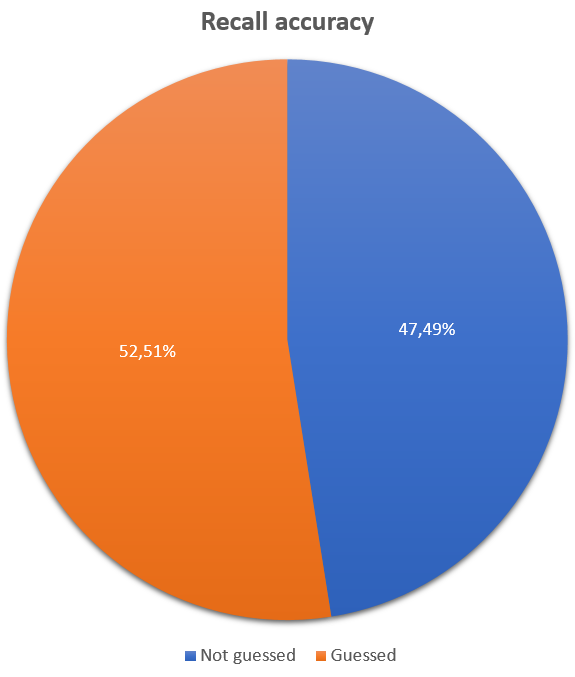
\includegraphics[scale=0.7]{recallAccuracy}
\caption{Recall accuracy}
\label{recallAccuracy}
\end{figure}
The percentage of how many times the recommendation engine would have predicted a visitors actual behavior is therefore \begin{math}2974/5664*100=52.5\%\end{math} the result of this evaluation as well as the scripts used can be found attached with the source code. \\
The engine only had half of each visitors behavior to go on which could be only 1 behavior and still managed to guess correctly more than half of the time. The 47.5\% of the time the algorithm did not correctly guess the behavior does not mean that these were bad recommendations - the visitors might not have discovered these items themselves but as they were recommended they might have examined these as well. The percentage of correct behaviors guessed would be even higher if more product recommendations where requested in the test. \\
As the algorithm acquires more data on all visitors as well as the visitor requesting recommendations the predictions will become even more precise.

\subsubsection{Online validation}
When the recommendation algorithm is put into production several new and better ways of evaluating the system becomes available. As the visitors get recommendations their behavior is logged and it is therefore easy to see how many of the recommendations are actually used and adjust the algorithm thereafter.
This adjustment can potentially be automatized by using machine learning.

\subsection{Concrete examples}
To give a better understanding of the recommendations given by the algorithm a few specific examples are given below. \\

\textbf{Visitor AAF995AE-1DD0-41C6-898B-9CBEE884E553} has looked at the following products:
\begin{itemize}
\item \textbf{36991: }Playset Brandmand Sam fyrtårn med figur
\item \textbf{37691: }Playset Brandmand Sam Havnestation
\item \textbf{37799: }Firman Sam Ocean Rescue
\item \textbf{38950: }Sejt Brandmand Sam udstyrssæt
\item \textbf{40786: }Brandmand Sam helikopter med lys og lyd
\item \textbf{42373: }Biler Brandmand Sam og brandbil
\item \textbf{52818: }Udklædning tilbehør sej Brandmand Sam megafon
\item \textbf{52919: }Playset Fireman Sam
\end{itemize}
and is recommended the following products:
\begin{itemize}
\item \textbf{43215: }Biler Brandmand Sam bil
\item \textbf{36991: }Payset Brandmand Sam fyrtårn med figur
\item \textbf{37799: }Firman Sam Ocean Rescue
\item \textbf{38950: }Sejt Brandmand Sam udstyrssæt med bælte
\item \textbf{34392:} Brandmand Sam 104 cm Fastelavnstøj
\end{itemize}

The visitor has already looked at some of the items recommended, but others he has not. As the recommendations size increases more new products to the visitor will appear. The recommendations seem valid since they are all "Brandmand Sam" stuff which is all he has looked at in the past. In the future the recommendation engine will be able to sort out his orders, but this has yet to be implemented. \\\\

Another \textbf{visitor 0036ECB4-F5AB-4B7C-824C-8D1C832CB65A} has looked at the following products:
\begin{itemize}
\item \textbf{43106: }Biler Scalextric C3528 BMW MINI Cooper S
\item \textbf{49777: }Scalextric Racerbane C1368 Bilbaner Le Mans Prototypes Sports Cars
\item \textbf{33136: }Chevrolet Camaro GT-R Biler Scalextric C3383 
\item \textbf{43104: }Scalextric C3524 VW Polo WRC Biler
\end{itemize}
and is recommended the following 5 products:
\begin{itemize}
\item \textbf{43106: }Biler Scalextric C3528 BMW MINI Cooper S
\item \textbf{43104: }Scalextric C3524 VW Polo WRC Biler
\item \textbf{49777: }Scalextric Racerbane C1368 Bilbaner Le Mans Prototypes Sports Cars
\item \textbf{33136: }Chevrolet Camaro GT-R Biler Scalextric C3383
\item \textbf{42841: }Maserati Trofeo Biler Scalextric C3388
\end{itemize}

These recommendations also look valid theme-wise as they relate closely to the products the visitor has viewed. \\\\

A final example \textbf{visitor 22C9CF0F-8B96-4764-A2D1-6194992CEDC2} has looked at these products:
\begin{itemize}
\item \textbf{42809: }Bosch arbejdsbord Bosch Værktøj og Værktøjsbænke
\item \textbf{42106: }Elsker du også bare paw patrol
\end{itemize}
and is recommended these products:
\begin{itemize}
\item \textbf{42106: }Elsker du også bare paw patrol
\item \textbf{42809: }Bosch arbejdsbord Bosch Værktøj og Værktøjsbænke
\item \textbf{40542: }LEGO Legends Of Chima Flyv op gennem skyerne
\item \textbf{31548:} LEGO Legends Of Chima Snurrende slyngplanter
\item \textbf{43713:} Fastelavnstøj Tid til at ringe efter politiet og Paw Patrols hund nummer 1
\end{itemize}
The two LEGO recommendations in this example might not seem thematically accurate, however since they have been recommended they must have a high similarity score to one or both of the products the visitor has looked at. A closer look at the data shows the two LEGO products to have similarity scores of 24 and 15 respectively to product 42106. Since these products are not in the same product group and have zero matching descriptions the high similarity score is the amount of times they have been looked at together with this product. The main product, product 42106, have been looked at by 9 other visitors and these 9 visitors have then looked at the first LEGO product 24 times and the second LEGO product 15 times.

\section{Conclusion}
The system has been validated statistically with the Recall method where the algorithm correctly predicted 52.5\% of the visitors' behavior which would be even higher if more recommendations were requested in the test.. Concrete examples have also been examined and the recommendations makes sense when looked at. A few other measures such as RMSE and MAE could not be used due to the lack of product rating from the visitors.

 